\documentclass[11pt,letterpaper]{article}
\usepackage[sinindice]{tecnm}
\usepackage{tikz}
\usetikzlibrary{arrows.meta,positioning,shapes.geometric}
\usepackage{booktabs,array,amsmath,amssymb}

\materia{Inteligencia Artificial y su Ética}
\actividad{Tema 2.1 - Actividad 8 \\ Introducción a los Algoritmos de Búsqueda}
\profesor{M. Lilia Ureña Lugo}

% Estilos visuales para los grafos de estados
\tikzset{
  inicio/.style={draw=blue!70!black,fill=blue!15,rounded corners=3pt,thick,align=center,font=\scriptsize,inner sep=4pt,minimum width=1.8cm},
  meta/.style={draw=green!50!black,fill=green!20,rounded corners=3pt,thick,align=center,font=\scriptsize,inner sep=4pt,minimum width=1.8cm},
  sol/.style={draw=orange!80!black,fill=orange!15,rounded corners=3pt,thick,align=center,font=\scriptsize,inner sep=4pt,minimum width=1.8cm},
  otro/.style={draw=gray!60,fill=gray!10,rounded corners=3pt,align=center,font=\scriptsize,inner sep=4pt,minimum width=1.8cm},
  solarco/.style={orange!90!black,very thick,-{Stealth[scale=1.1]}},
  otroarco/.style={gray!60,-{Stealth}},
  paso/.style={circle,fill=white,draw=orange!90!black,font=\scriptsize\bfseries,inner sep=1.5pt}
}

\begin{document}
\portada
\indicegeneral

\section{Introducción}

En el ámbito de la Inteligencia Artificial, la resolución de problemas mediante algoritmos de búsqueda requiere formalizar el entorno a través de cuatro elementos fundamentales:

\begin{itemize}
  \item \textbf{Estado inicial (nodo inicial):} Configuración o punto de partida del sistema antes de ejecutar cualquier acción.
  \item \textbf{Estado meta (nodo meta):} Configuración o conjunto de condiciones objetivo que se desean alcanzar.
  \item \textbf{Acciones (u operadores):} Conjunto de transiciones válidas o transformaciones permitidas para pasar de un estado a otro.
  \item \textbf{Espacio de estados:} Estructura matemática (representada comúnmente como un grafo o árbol) formada por el conjunto de todos los estados alcanzables a partir del estado inicial mediante la aplicación de las acciones permitidas.
\end{itemize}

A continuación se presenta la descripción en lenguaje natural, la formalización matemática, la representación gráfica del espacio de estados/secuencia de búsqueda y el recorrido de solución detallado para los tres problemas establecidos.

%% ===================== EJERCICIO 1 =====================
\section{Ejercicio 1: Las jarras de agua}

\subsection{Descripción en lenguaje natural}
\begin{itemize}
  \item \textbf{Estado inicial:} Dos jarras vacías: una con capacidad de 4 litros (J4) y otra de 3 litros (J3).
  \item \textbf{Estado meta:} La jarra de 4 litros contiene exactamente 2 litros de agua $(x = 2)$, independientemente de la cantidad retenida en la jarra de 3 litros.
  \item \textbf{Acciones:} Llenar completamente cualquiera de las dos jarras desde el grifo; vaciar totalmente cualquier jarra al suelo; o verter el contenido de una jarra en la otra hasta llenar la receptora o vaciar la emisora.
  \item \textbf{Espacio de estados:} Todas las combinaciones de volúmenes enteros $(x, y)$ alcanzables con $0 \le x \le 4$ y $0 \le y \le 3$.
\end{itemize}

\subsection{Representación formal}
Un estado se define como el par ordenado $(x, y)$, donde $x \in \{0,1,2,3,4\}$ representa los litros contenidos en J4, y $y \in \{0,1,2,3\}$ representa los litros contenidos en J3.

\begin{itemize}
  \item \textbf{Espacio de estados:} $S = \{(x,y) \in \mathbb{Z}^2 \mid 0 \le x \le 4, \, 0 \le y \le 3\}$.
  \item \textbf{Estado inicial:} $s_0 = (0,0)$.
  \item \textbf{Estados meta:} $G = \{(2,y) \mid 0 \le y \le 3\}$.
  \item \textbf{Acciones permitidas:}
\end{itemize}

\begin{center}
\small
\renewcommand{\arraystretch}{1.2}
\begin{tabular}{@{}lll@{}}
\toprule
\textbf{Operador} & \textbf{Acción} & \textbf{Transformación del estado $(x,y)$} \\
\midrule
$A_1$ & Llenar J4 & $(4, y)$ \\
$A_2$ & Llenar J3 & $(x, 3)$ \\
$A_3$ & Vaciar J4 & $(0, y)$ \\
$A_4$ & Vaciar J3 & $(x, 0)$ \\
$A_5$ & Verter J4 $\to$ J3 & $(x - t, y + t)$, donde $t = \min(x, 3-y)$ \\
$A_6$ & Verter J3 $\to$ J4 & $(x + t, y - t)$, donde $t = \min(y, 4-x)$ \\
\bottomrule
\end{tabular}
\end{center}

\subsection{Grafo / Diagrama de estados y recorrido de solución}

Siguiendo la secuencia de solución estudiada en clase, la Figura~\ref{fig:jarras} ilustra la transición de estados que conduce al estado meta $(2,0)$, y la Tabla~\ref{tab:jarras} desglosa las acciones aplicadas.

\begin{figure}[ht]
\centering
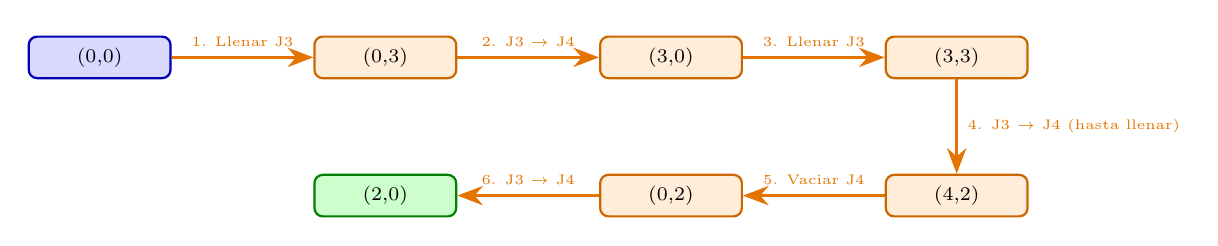
\begin{tikzpicture}[node distance=1.2cm and 1.8cm, auto]
\node[inicio] (e0) {(0,0)};
\node[sol, right=of e0] (e1) {(0,3)};
\node[sol, right=of e1] (e2) {(3,0)};
\node[sol, right=of e2] (e3) {(3,3)};
\node[sol, below=1.2cm of e3] (e4) {(4,2)};
\node[sol, left=of e4] (e5) {(0,2)};
\node[meta, left=of e5] (e6) {(2,0)};

\draw[solarco] (e0) -- node[above,font=\tiny]{1. Llenar J3} (e1);
\draw[solarco] (e1) -- node[above,font=\tiny]{2. J3 $\to$ J4} (e2);
\draw[solarco] (e2) -- node[above,font=\tiny]{3. Llenar J3} (e3);
\draw[solarco] (e3) -- node[right,font=\tiny]{4. J3 $\to$ J4 (hasta llenar)} (e4);
\draw[solarco] (e4) -- node[above,font=\tiny]{5. Vaciar J4} (e5);
\draw[solarco] (e5) -- node[above,font=\tiny]{6. J3 $\to$ J4} (e6);
\end{tikzpicture}
\caption{Diagrama de transición de estados para el problema de las jarras. Elaboración propia.}
\label{fig:jarras}
\end{figure}

\begin{table}[ht]
\centering\small
\renewcommand{\arraystretch}{1.15}
\begin{tabular}{@{}clcc@{}}
\toprule
\textbf{Paso} & \textbf{Acción ejecutada} & \textbf{Estado origen} & \textbf{Estado destino} \\
\midrule
1 & Llenar la jarra de 3 L & (0,0) & (0,3) \\
2 & Pasar agua de jarra de 3 L a jarra de 4 L & (0,3) & (3,0) \\
3 & Volver a llenar la jarra de 3 L & (3,0) & (3,3) \\
4 & Pasar agua de 3 L a 4 L hasta llenarla & (3,3) & (4,2) \\
5 & Vaciar la jarra de 4 L & (4,2) & (0,2) \\
6 & Pasar los 2 L restantes de 3 L a 4 L & (0,2) & (2,0) \\
\bottomrule
\end{tabular}
\caption{Secuencia detallada de pasos para la resolución del problema de las jarras. Elaboración propia.}
\label{tab:jarras}
\end{table}

%% ===================== EJERCICIO 2 =====================
\section{Ejercicio 2: El pastor, el lobo, la cabra y la lechuga}

\subsection{Descripción en lenguaje natural}
\begin{itemize}
  \item \textbf{Estado inicial:} El pastor, el lobo, la cabra y la lechuga están reunidos en la orilla A del río.
  \item \textbf{Estado meta:} Los cuatro elementos han cruzado a la orilla B.
  \item \textbf{Acciones:} El pastor cruza en el bote hacia la orilla opuesta solo o transportando un único elemento (lobo, cabra o lechuga) que se encuentre en su misma orilla.
  \item \textbf{Espacio de estados:} Combinaciones de ubicación seguras donde nunca queden en la misma orilla el lobo con la cabra sin el pastor, ni la cabra con la lechuga sin el pastor.
\end{itemize}

\subsection{Representación formal}
Un estado se representa como la tupla $(p, l, c, h) \in \{0,1\}^4$, donde la variable toma el valor $0$ si está en la orilla A y $1$ si está en la B ($p$: pastor, $l$: lobo, $c$: cabra, $h$: lechuga).

\begin{itemize}
  \item \textbf{Espacio de estados:} $S = \{(p,l,c,h) \in \{0,1\}^4 \mid (l = c \implies p = l) \land (c = h \implies p = c)\}$. Existen 10 estados válidos.
  \item \textbf{Estado inicial:} $s_0 = (0,0,0,0)$.
  \item \textbf{Estado meta:} $G = \{(1,1,1,1)\}$.
  \item \textbf{Acciones:} Cambio de orilla del pastor ($p' = 1 - p$) transportando opcionalmente un elemento $x \in \{l, c, h\}$ presente en su misma orilla.
\end{itemize}

\subsection{Grafo de estados y secuencia de solución}

\begin{figure}[ht]
\centering
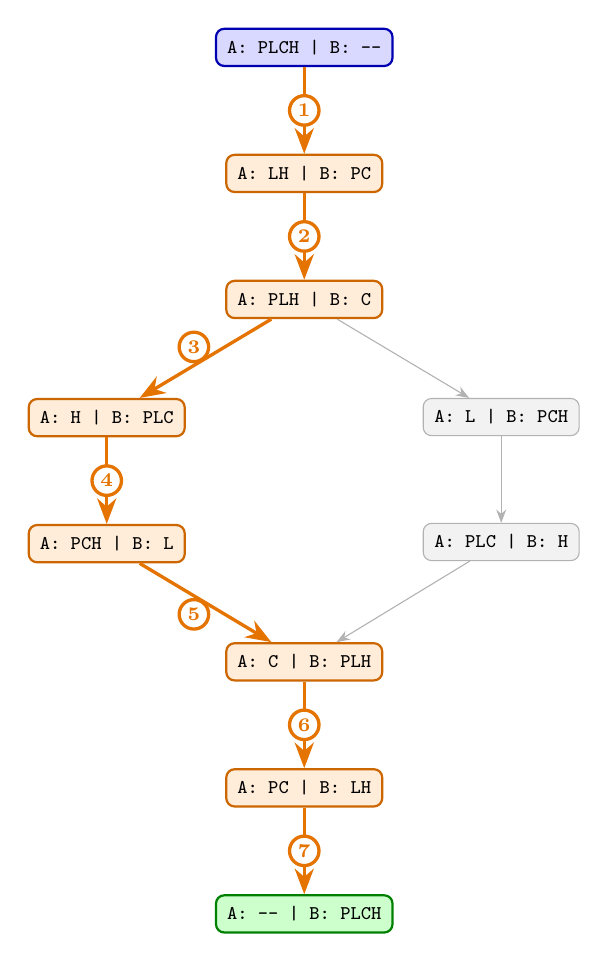
\begin{tikzpicture}[node distance=1.1cm]
\node[inicio] (n0) {\texttt{A: PLCH | B: --}};
\node[sol, below=of n0] (n1) {\texttt{A: LH   | B: PC}};
\node[sol, below=of n1] (n2) {\texttt{A: PLH  | B: C}};
\node[sol, below left=1cm and 0.5cm of n2] (n3a) {\texttt{A: H    | B: PLC}};
\node[otro, below right=1cm and 0.5cm of n2] (n3b) {\texttt{A: L    | B: PCH}};
\node[sol, below=of n3a] (n4a) {\texttt{A: PCH  | B: L}};
\node[otro, below=of n3b] (n4b) {\texttt{A: PLC  | B: H}};
\node[sol, below right=1cm and 0.5cm of n4a] (n5) {\texttt{A: C    | B: PLH}};
\node[sol, below=of n5] (n6) {\texttt{A: PC   | B: LH}};
\node[meta, below=of n6] (n7) {\texttt{A: --   | B: PLCH}};

\draw[solarco] (n0) -- node[paso]{1} (n1);
\draw[solarco] (n1) -- node[paso]{2} (n2);
\draw[solarco] (n2) -- node[paso,above left]{3} (n3a);
\draw[otroarco] (n2) -- (n3b);
\draw[solarco] (n3a) -- node[paso]{4} (n4a);
\draw[otroarco] (n3b) -- (n4b);
\draw[solarco] (n4a) -- node[paso,below left]{5} (n5);
\draw[otroarco] (n4b) -- (n5);
\draw[solarco] (n5) -- node[paso]{6} (n6);
\draw[solarco] (n6) -- node[paso]{7} (n7);
\end{tikzpicture}
\caption{Grafo completo del espacio de estados del problema del pastor con el camino óptimo enmarcado. Elaboración propia.}
\label{fig:pastor}
\end{figure}

\begin{table}[ht]
\centering\small
\renewcommand{\arraystretch}{1.15}
\begin{tabular}{@{}clcc@{}}
\toprule
\textbf{Paso} & \textbf{Acción (Cruzar)} & \textbf{Estado inicial tupla} & \textbf{Estado resultante tupla} \\
\midrule
1 & Pastor cruza con la Cabra (A $\to$ B) & (0,0,0,0) & (1,0,1,0) \\
2 & Pastor regresa solo (B $\to$ A) & (1,0,1,0) & (0,0,1,0) \\
3 & Pastor cruza con el Lobo (A $\to$ B) & (0,0,1,0) & (1,1,1,0) \\
4 & Pastor regresa con la Cabra (B $\to$ A) & (1,1,1,0) & (0,1,0,0) \\
5 & Pastor cruza con la Lechuga (A $\to$ B) & (0,1,0,0) & (1,1,0,1) \\
6 & Pastor regresa solo (B $\to$ A) & (1,1,0,1) & (0,1,0,1) \\
7 & Pastor cruza con la Cabra (A $\to$ B) & (0,1,0,1) & (1,1,1,1) \\
\bottomrule
\end{tabular}
\caption{Secuencia optima de solución para el cruce del río. Elaboración propia.}
\label{tab:pastor}
\end{table}

%% ===================== EJERCICIO 3 =====================
\section{Ejercicio 3: Misioneros y caníbales}

\subsection{Descripción en lenguaje natural}
\begin{itemize}
  \item \textbf{Estado inicial:} 3 misioneros, 3 caníbales y la barca en la orilla A.
  \item \textbf{Estado meta:} Todos (3 misioneros, 3 caníbales y la barca) han cruzado a la orilla B.
  \item \textbf{Acciones:} Trasladar en la barca a 1 o 2 personas por viaje (en cualquier combinación de roles), siempre garantizando la presencia de al menos 1 tripulante.
  \item \textbf{Espacio de estados:} Conjunto de distribuciones válidas donde, en ninguna de las dos orillas, la cantidad de caníbales sea superior a la de misioneros (salvo cuando el número de misioneros en dicha orilla sea 0).
\end{itemize}

\subsection{Representación formal}
Un estado se define como la tupla $(m, c, b)$, donde $m, c \in \{0,1,2,3\}$ representan el número de misioneros y caníbales en la orilla A, y $b \in \{A, B\}$ indica la posición actual de la barca. En la orilla B habrá $(3-m)$ misioneros y $(3-c)$ caníbales.

\begin{itemize}
  \item \textbf{Espacio de estados:} 
  $$S = \{(m,c,b) \mid (m = 0 \lor m \ge c) \land (3-m = 0 \lor 3-m \ge 3-c)\}$$
  \item \textbf{Estado inicial:} $s_0 = (3,3,A)$.
  \item \textbf{Estado meta:} $G = \{(0,0,B)\}$.
  \item \textbf{Acciones:} Trasladar $(d_m, d_c)$ con $1 \le d_m + d_c \le 2$.
\end{itemize}

\subsection{Grafo de estados y secuencia de solución}

\begin{figure}[ht]
\centering
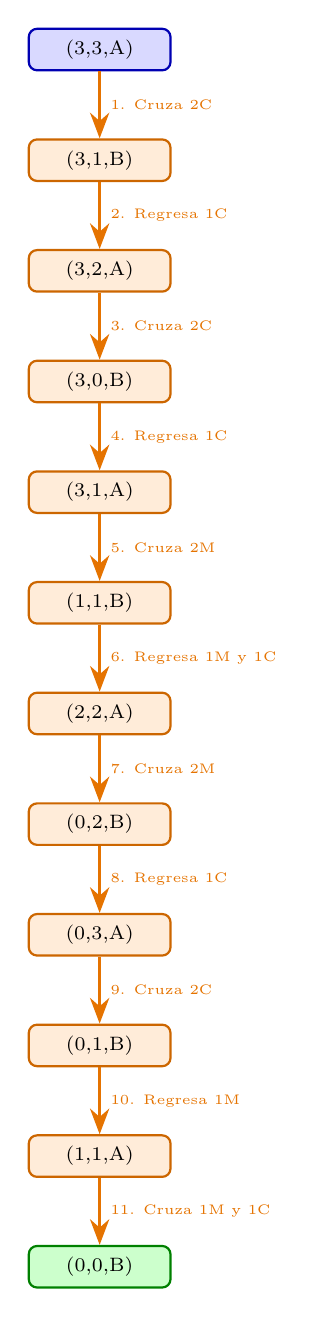
\begin{tikzpicture}[node distance=0.85cm]
\node[inicio] (s0) {(3,3,A)};
\node[sol, below=of s0] (s1) {(3,1,B)};
\node[sol, below=of s1] (s2) {(3,2,A)};
\node[sol, below=of s2] (s3) {(3,0,B)};
\node[sol, below=of s3] (s4) {(3,1,A)};
\node[sol, below=of s4] (s5) {(1,1,B)};
\node[sol, below=of s5] (s6) {(2,2,A)};
\node[sol, below=of s6] (s7) {(0,2,B)};
\node[sol, below=of s7] (s8) {(0,3,A)};
\node[sol, below=of s8] (s9) {(0,1,B)};
\node[sol, below=of s9] (s10) {(1,1,A)};
\node[meta, below=of s10] (s11) {(0,0,B)};

\draw[solarco] (s0) -- node[right,font=\tiny]{1. Cruza 2C} (s1);
\draw[solarco] (s1) -- node[right,font=\tiny]{2. Regresa 1C} (s2);
\draw[solarco] (s2) -- node[right,font=\tiny]{3. Cruza 2C} (s3);
\draw[solarco] (s3) -- node[right,font=\tiny]{4. Regresa 1C} (s4);
\draw[solarco] (s4) -- node[right,font=\tiny]{5. Cruza 2M} (s5);
\draw[solarco] (s5) -- node[right,font=\tiny]{6. Regresa 1M y 1C} (s6);
\draw[solarco] (s6) -- node[right,font=\tiny]{7. Cruza 2M} (s7);
\draw[solarco] (s7) -- node[right,font=\tiny]{8. Regresa 1C} (s8);
\draw[solarco] (s8) -- node[right,font=\tiny]{9. Cruza 2C} (s9);
\draw[solarco] (s9) -- node[right,font=\tiny]{10. Regresa 1M} (s10);
\draw[solarco] (s10) -- node[right,font=\tiny]{11. Cruza 1M y 1C} (s11);
\end{tikzpicture}
\caption{Secuencia de solución en el espacio de estados de Misioneros y Caníbales. Elaboración propia.}
\label{fig:misioneros}
\end{figure}

\begin{table}[ht]
\centering\small
\renewcommand{\arraystretch}{1.15}
\begin{tabular}{@{}clcc@{}}
\toprule
\textbf{Paso} & \textbf{Cruce realizado} & \textbf{Estado Origen $(m,c,b)$} & \textbf{Estado Destino $(m,c,b)$} \\
\midrule
1 & 0 Misioneros + 2 Caníbales (A $\to$ B) & (3,3,A) & (3,1,B) \\
2 & 0 Misioneros + 1 Caníbal (B $\to$ A) & (3,1,B) & (3,2,A) \\
3 & 0 Misioneros + 2 Caníbales (A $\to$ B) & (3,2,A) & (3,0,B) \\
4 & 0 Misioneros + 1 Caníbal (B $\to$ A) & (3,0,B) & (3,1,A) \\
5 & 2 Misioneros + 0 Caníbales (A $\to$ B) & (3,1,A) & (1,1,B) \\
6 & 1 Misionero + 1 Caníbal (B $\to$ A) & (1,1,B) & (2,2,A) \\
7 & 2 Misioneros + 0 Caníbales (A $\to$ B) & (2,2,A) & (0,2,B) \\
8 & 0 Misioneros + 1 Caníbal (B $\to$ A) & (0,2,B) & (0,3,A) \\
9 & 0 Misioneros + 2 Caníbales (A $\to$ B) & (0,3,A) & (0,1,B) \\
10 & 1 Misionero + 0 Caníbales (B $\to$ A) & (0,1,B) & (1,1,A) \\
11 & 1 Misionero + 1 Caníbal (A $\to$ B) & (1,1,A) & (0,0,B) \\
\bottomrule
\end{tabular}
\caption{Camino óptimo de 11 pasos para el problema de misioneros y caníbales. Elaboración propia.}
\label{tab:misioneros}
\end{table}

\section{Conclusión}
La formalización matemática y la construcción del grafo del espacio de estados resultan indispensables para aplicar algoritmos de búsqueda en Inteligencia Artificial. Al descomponer el problema en sus componentes fundamentales, es posible garantizar una búsqueda sistemática y encontrar la secuencia de transiciones mínima necesaria para alcanzar el estado meta.

\referencias
\end{document}